\documentclass{article}
\usepackage{hyperref}
\usepackage{amsmath,amssymb}
\usepackage{graphicx}
\usepackage{algorithm,algorithmic}
\usepackage[a4paper,margin=1in]{geometry}

\newcommand{\encP}[1]{\emph{enc}^{\mathrm{poly}}\!\left(#1\right)}
\newcommand{\ser}[1]{\emph{ser}^{\mathrm{bin}}\!\left(#1\right)}
\newcommand{\encB}[1]{\emph{enc}^{\mathrm{B64}}\!\left(#1\right)}
\newcommand{\selMinLogN}[1]{\mathsf{selMinLogN}\!\left(#1\right)}
\newcommand{\selParams}[1]{\mathsf{selParams}\!\left(#1\right)}
\newcommand{\genRecords}[1]{\mathsf{genRecords}\!\left(#1\right)}
\newcommand{\feasible}[1]{\mathsf{feasible}\!\left(#1\right)}

\begin{document}

\title{Supplementary Material for\\``TWAPPA-FRL: Trust-Weighted Privacy-Preserving Aggregation for Federated Reinforcement Learning in Collaborative Intrusion Detection''}
\author{Piyumi M. S. Rajapaksha \and Artur Iasenovets \and Yinxue Yi \and Fei Tang}
\date{}
\maketitle

\section{Detailed Algorithms}
This section provides the workflow algorithms for the $ep_{\mathrm{twa\text{-}ppa}}$ execution path.

\subsection{TWA Component Definitions}\label{sec:supp_twa_components}

Let
\[
\operatorname{clip}_{[0,1]}(x)=\min(1,\max(0,x)).
\]
The fixed public protocol constant $\delta_0=10^{-8}$ is the numerical
stabilizer.
The parameter domains are $\alpha_k\geq0$ with $\sum_k\alpha_k=1$,
$\beta,\lambda\in[0,1]$, $\rho\geq0$, $\tau>0$, $r_{\max}>r_{\min}$,
$w_{\max}>0$, and $C>0$.

For per-step rewards in $[-2,3]$ and at most $t_{\max}$ steps per episode,
$r_{\min}=-2t_{\max}$ and $r_{\max}=3t_{\max}$. For the reported
five-client configuration $t_{\max}=16$, hence
$(r_{\min},r_{\max})=(-32,48)$.

For the latest reward-history window
$\mathcal H_{\mathrm{rew},i}^{(r)}=
(\bar r_i^{(t)})_{t=\max(0,r-4)}^{r}$, reward stability is
\[
s_i^{\mathrm{raw}}=
\begin{cases}
0.7, & |\mathcal H_{\mathrm{rew},i}^{(r)}|<2,\\
\operatorname{clip}_{[0,1]}
\left[
\dfrac{1}{1+
\operatorname{std}(\mathcal H_{\mathrm{rew},i}^{(r)})/
(\operatorname{mean}|\mathcal H_{\mathrm{rew},i}^{(r)}|+\delta_0)}
\right], & \text{otherwise,}
\end{cases}
\qquad
S_i=s_i^{\mathrm{raw}}.
\]
For a window $\mathcal H$ of length $n$, the calculation uses the population
standard deviation
\[
\operatorname{std}(\mathcal H)=
\left[n^{-1}\sum_{x\in\mathcal H}
(x-\operatorname{mean}(\mathcal H))^2\right]^{1/2}.
\]
The quality component is
$Q_i=\operatorname{clip}_{[0,1]}((\bar r_i-r_{\min})/(r_{\max}-r_{\min}))$.
For the clipped update $\mathbf z_i$ and the reference update
$\mathbf v=\mathsf{flatten}(\Delta\theta_{\mathrm{agg}}^{(r-1)})$,
\[
M_i=\operatorname{clip}_{[0,1]}
\left(
\dfrac{1}{2}\left[
1+\dfrac{\mathbf z_i^\top\mathbf v}
{\|\mathbf z_i\|_2\cdot\|\mathbf v\|_2+\delta_0}
\right]
\right),
\qquad
H_i=
\begin{cases}
0.5, & b_i^{(r)}=1,\\
T_i^{(r-1)}, & b_i^{(r)}=0,
\end{cases}.
\]
Let $\mathcal I_{r-1}$ be the set of client indices for which $\mathcal{TC}$
stores a prior trust value. Then $b_i^{(r)}=1$ exactly when
$i\notin\mathcal I_{r-1}$, and $b_i^{(r)}=0$ otherwise.
If local validation data $\mathcal V_i$ are available,
$\mathsf{LocalF1Metric}(\mathcal V_i)$ is the macro-F1 score
\[
F_i^{\mathrm{raw}}=
\dfrac{1}{J}\sum_{c=1}^{J}
\dfrac{2p_{i,c}q_{i,c}}{p_{i,c}+q_{i,c}},
\]
where $p_{i,c}$ and $q_{i,c}$ are class-$c$ precision and recall; a term is
zero when its denominator is zero. Otherwise, $F_i^{\mathrm{raw}}=0.5$, and
$F_i=\operatorname{clip}_{[0,1]}(F_i^{\mathrm{raw}})$. Finally,
\[
d_i=\dfrac{|g_i-g_{\mathrm{med}}|}{g_{\mathrm{med}}+\delta_0},
\qquad
G_i=\dfrac{1}{1+d_i}.
\]
These local transforms define the distributed protocol.

\subsection{Protocol Algorithms}\label{sec:supp_protocol_algorithms}

For compact workflow notation, let
\[
\mathcal X_i^{(r)}=
\left(\Delta\theta_i^{(r)},|\mathcal D_i|,\bar r_i,
\mathcal H_{\mathrm{rew},i}^{(r)},F_i^{\mathrm{raw}},g_i,g_{\mathrm{med}},
\Delta\theta_{\mathrm{agg}}^{(r-1)},T_i^{(r-1)},b_i^{(r)}\right).
\]
The following algorithms use these definitions when invoking
\textsc{TrustScore}.
Before round $0$, initialize the public aggregate state
$\Delta\theta_{\mathrm{agg}}^{(-1)}=\mathbf0$, the stored-client index set
$\mathcal I_{-1}=\varnothing$, and each client-local reward history
$\mathcal H_{\mathrm{rew},i}^{(-1)}=[\,]$.

\setcounter{algorithm}{0}
\renewcommand{\thealgorithm}{S\arabic{algorithm}}

\begin{algorithm}[H]
  \caption{\textsc{TWA-PPA Workflow} --- $ep_{\mathrm{twa\text{-}ppa}}$ main path}
  \label{alg:frl}
    \begin{algorithmic}[1]
    \REQUIRE $\theta^{(r)}$; $\Delta\theta_{\mathrm{agg}}^{(r-1)}$;
    $pk$; $\mathrm{pp}$; $sk$
    \REQUIRE $\mathcal I_{r-1}$;
    $\{T_i^{(r-1)}\}_{i\in\mathcal I_{r-1}}$;
    $\{\alpha_k,\beta,\lambda,\rho,\tau,r_{\min},r_{\max},w_{\max},C\}$;
    \REQUIRE
    $\{(\mathcal{DC}_i,\mathcal{E}_i,\mathcal{D}_i,\mathcal{V}_i)\}_{i=1}^{K}$
    \ENSURE $\theta^{(r+1)}$

    \STATE \textbf{Broadcast} $\theta^{(r)}$ and the public
    $\Delta\theta_{\mathrm{agg}}^{(r-1)}$ to all $\mathcal{DC}_i$

    \FOR{each client $i \in \{1,\ldots,K\}$ \textbf{in parallel}}
      \STATE $(\Delta\theta_i^{(r)},\bar{r}_i,\bar{\ell}_i)
      \leftarrow \textsc{LocalTrain}(\theta^{(r)},E,\mathcal{E}_i,\mathcal{D}_i)$
      \STATE $\mathcal H_{\mathrm{rew},i}^{(r)}\leftarrow
      \mathsf{tail}_5(\mathcal H_{\mathrm{rew},i}^{(r-1)}
      \mathbin{\|}[\bar r_i])$ locally
      \STATE $F_i^{\mathrm{raw}}\leftarrow\mathsf{LocalF1Metric}(\mathcal{V}_i)$ if available; otherwise $F_i^{\mathrm{raw}}\leftarrow0.5$
      \STATE $g_i\leftarrow\|\mathsf{flatten}(\Delta\theta_i^{(r)})\|_2$
    \ENDFOR

    \STATE $\mathcal{TC}$ receives $\{g_i\}_{i=1}^{K}$
    \STATE $\mathcal{TC}$ sets $b_i^{(r)}\leftarrow1$ if
    $i\notin\mathcal I_{r-1}$, and $b_i^{(r)}\leftarrow0$ otherwise
    \STATE $\mathcal{TC}$ sets $T_i^{(r-1)}\leftarrow0.5$ when $b_i^{(r)}=1$
    \STATE $g_{\mathrm{med}}\leftarrow\mathsf{median}(\{g_i\}_{i=1}^{K})$
    \STATE $\mathcal{TC}$ distributes $g_{\mathrm{med}}$ to all $\mathcal{DC}_i$
    \STATE $\mathcal{TC}$ provides $(T_i^{(r-1)},b_i^{(r)})$ to each
    $\mathcal{DC}_i$

    \FOR{each client $i \in \{1,\ldots,K\}$ \textbf{in parallel}}
      \STATE $(\bar{\Delta\theta}_i^{(r)},\hat{w}_i^{(r)},T_i^{(r)})
      \leftarrow\textsc{TrustScore}
      (\mathcal X_i^{(r)},\Phi_{\mathrm{TWA}})$
    \ENDFOR

    \STATE Each $\mathcal{DC}_i$ sends
    $T_i^{(r)}$ directly to $\mathcal{TC}$
    \STATE Each $\mathcal{DC}_i$ sends
    $(\hat{w}_i^{(r)},|\mathcal{D}_i|)$ to $\mathcal{AC}$
    \STATE $\mathcal{TC}$ stores
    $\{T_i^{(r)}\}_{i=1}^{K}$ for use as the previous trust state in round $r+1$
    \STATE $\{w_i^{(r)}\}_{i=1}^{K}
    \leftarrow \textsc{TrustWeightNorm}
    (\{\hat{w}_i^{(r)}\}_{i=1}^{K},
    \{|\mathcal{D}_i|\}_{i=1}^{K},w_{\max})$

    \FOR{each client $i \in \{1,\ldots,K\}$ \textbf{in parallel}}
      \STATE $\{\mathsf{ct}_{i,\ell}^{(r)}\}_{\ell=0}^{L-1}
      \leftarrow \textsc{CKKSEncryptDelta} (\bar{\Delta\theta}_i^{(r)},pk,P,m_{\mathrm{slot}})$

    \ENDFOR

    \STATE Each $\mathcal{DC}_i$ sends
    $\{\mathsf{ct}_{i,\ell}^{(r)}\}_{\ell=0}^{L-1}$ to $\mathcal{AC}$

    \STATE $\{\mathsf{ct}_{\mathrm{agg},\ell}^{(r)}\}_{\ell=0}^{L-1}
    \leftarrow \textsc{HEWeightedAggregate}
    (\{\mathsf{ct}_{i,\ell}^{(r)}\},\{w_i^{(r)}\},\mathrm{pp})$

    \STATE $\mathcal{AC}$ sends only
    $\{\mathsf{ct}_{\mathrm{agg},\ell}^{(r)}\}_{\ell=0}^{L-1}$
    to $\mathcal{KA}$

    \STATE $\Delta\theta_{\mathrm{HE}}^{(r)}
    \leftarrow \textsc{DecryptAggregate}
    (\{\mathsf{ct}_{\mathrm{agg},\ell}^{(r)}\}_{\ell=0}^{L-1},
    sk,P,m_{\mathrm{slot}})$

    \STATE $\mathcal{KA}$ returns
    $\Delta\theta_{\mathrm{HE}}^{(r)}$ to $\mathcal{AC}$

    \STATE $\Delta\theta_{\mathrm{agg}}^{(r)}
    \leftarrow \Delta\theta_{\mathrm{HE}}^{(r)}$

    \STATE $\theta^{(r+1)}
    \leftarrow \theta^{(r)}+\Delta\theta_{\mathrm{agg}}^{(r)}$

    \STATE \textbf{Broadcast} $\theta^{(r+1)}$ to all $\mathcal{DC}_i$
    \STATE \textbf{Log} accuracy, macro-F1, reward
    \STATE \textbf{return} $\theta^{(r+1)}$
    \end{algorithmic}
\end{algorithm}

\begin{algorithm}[H]
  \caption{\textsc{LocalTrain} at $\mathcal{DC}_i$}
  \label{alg:localtrain}
  \begin{algorithmic}[1]
  \REQUIRE $\theta^{(r)}$; $E$; $\mathcal{E}_i$; $\mathcal{D}_i$
  \ENSURE $\Delta\theta_i^{(r)}$; $\bar{r}_i$; $\bar{\ell}_i$
  \STATE $\theta_i \leftarrow \theta^{(r)}$; $\mathcal{R}_{\mathrm{ep}}\leftarrow[\,]$; $\mathcal{L}_{\mathrm{train}}\leftarrow[\,]$
  \FOR{$e=1,\ldots,E$}
    \STATE $s\leftarrow\mathcal{E}_i.\mathsf{reset}()$; $d\leftarrow\mathsf{false}$; $r_e\leftarrow0$; $t\leftarrow0$
    \WHILE{$\neg d \wedge t<t_{\max}$}
      \STATE $a\leftarrow\pi_i^{\varepsilon\text{-greedy}}(s;\theta_i)$
      \STATE $(s',r,d)\leftarrow\mathcal{E}_i.\mathsf{step}(a)$
      \STATE $\mathcal{D}_i.\mathsf{store}(s,a,r,s',d)$
      \STATE $\ell_{\mathrm{loss}}\leftarrow\mathsf{DQNTrainStep}(\theta_i,\mathcal{D}_i)$
      \IF{$\ell_{\mathrm{loss}}\neq\varnothing$}
        \STATE $\mathcal{L}_{\mathrm{train}}.\mathsf{append}(\ell_{\mathrm{loss}})$
      \ENDIF
      \STATE $r_e\leftarrow r_e+r$; $s\leftarrow s'$; $t\leftarrow t+1$
    \ENDWHILE
    \STATE $\mathcal{R}_{\mathrm{ep}}.\mathsf{append}(r_e)$
  \ENDFOR
  \STATE $\Delta\theta_i^{(r)}\leftarrow\theta_i^{\mathrm{local}}-\theta^{(r)}$
  \STATE $\bar{r}_i\leftarrow\mathsf{mean}(\mathcal{R}_{\mathrm{ep}})$; $\bar{\ell}_i\leftarrow\mathsf{mean}(\mathcal{L}_{\mathrm{train}})$
  \STATE \textbf{return} $(\Delta\theta_i^{(r)},\bar{r}_i,\bar{\ell}_i)$
  \end{algorithmic}
\end{algorithm}

\begin{algorithm}[H]
  \caption{\textsc{TrustScore} for client $i$}
  \label{alg:trust_score}
  \begin{algorithmic}[1]
  \REQUIRE $\Delta\theta_i^{(r)}$; $|\mathcal{D}_i|$; $\bar r_i$;
  $\mathcal H_{\mathrm{rew},i}^{(r)}$; $F_i^{\mathrm{raw}}$; $g_i$;
  $g_{\mathrm{med}}$; $\Delta\theta_{\mathrm{agg}}^{(r-1)}$;
  $T_i^{(r-1)}$; $b_i^{(r)}$;
  $\{\alpha_k,\beta,\lambda,\rho,\tau,r_{\min},r_{\max},w_{\max},C\}$
  \ENSURE $\bar{\Delta\theta}_i^{(r)}$; $\hat w_i$; $T_i$

  \STATE $\mathbf{z}_i\leftarrow\mathsf{flatten}(\Delta\theta_i^{(r)})$
  \IF{$\|\mathbf{z}_i\|_2>0$}
    \STATE $\mathbf{z}_i\leftarrow
    \mathbf{z}_i\cdot\min(1,C/\|\mathbf{z}_i\|_2)$
  \ELSE
    \STATE $\mathbf{z}_i\leftarrow\mathbf0$
  \ENDIF

  \STATE Compute $s_i^{\mathrm{raw}}$ from
  $\mathcal H_{\mathrm{rew},i}^{(r)}$;
  $S_i\leftarrow s_i^{\mathrm{raw}}$
  \STATE $Q_i\leftarrow\operatorname{clip}_{[0,1]}
  ((\bar r_i-r_{\min})/(r_{\max}-r_{\min}))$
  \STATE $\mathbf v\leftarrow
  \mathsf{flatten}(\Delta\theta_{\mathrm{agg}}^{(r-1)})$;
  $M_i\leftarrow\operatorname{clip}_{[0,1]}\bigl(
  \tfrac{1}{2}[1+\mathbf{z}_i^\top\mathbf v/
  (\|\mathbf{z}_i\|_2\cdot\|\mathbf v\|_2+\delta_0)]\bigr)$
  \STATE $H_i\leftarrow0.5$ if $b_i^{(r)}=1$; otherwise
  $H_i\leftarrow T_i^{(r-1)}$
  \STATE $F_i\leftarrow\operatorname{clip}_{[0,1]}(F_i^{\mathrm{raw}})$
  \STATE $d_i\leftarrow|g_i-g_{\mathrm{med}}|/
  (g_{\mathrm{med}}+\delta_0)$;
  $G_i\leftarrow1/(1+d_i)$

  \STATE $T_{i,\mathrm{raw}}\leftarrow
  \alpha_S S_i+\alpha_Q Q_i+\alpha_M M_i+\alpha_H H_i+\alpha_F F_i+\alpha_G G_i$
  \STATE $T_i\leftarrow T_{i,\mathrm{raw}}$ if $b_i^{(r)}=1$; otherwise
  $T_i\leftarrow\beta T_i^{(r-1)}+(1-\beta)T_{i,\mathrm{raw}}$

  \STATE $\bar{\Delta\theta}_i^{(r)}
  \leftarrow\mathsf{unflatten}(\mathbf{z}_i)$

  \IF{$T_i<\lambda$}
  \STATE $\hat w_i\leftarrow0$
  \ELSE
  \STATE $\hat w_i\leftarrow|\mathcal{D}_i|T_i^{\rho/\tau}$
  \ENDIF

  \STATE \textbf{return}
  $(\bar{\Delta\theta}_i^{(r)},\hat w_i,T_i)$
  \end{algorithmic}
\end{algorithm}

\begin{algorithm}[H]
  \caption{\textsc{TrustWeightNorm}}
  \label{alg:trust_weight_norm}
  \begin{algorithmic}[1]
  \REQUIRE $\{\hat w_i\}_{i=1}^{K}$;
  $\{|\mathcal{D}_i|\}_{i=1}^{K}$;
  $w_{\max}>0$
  \ENSURE $\{w_i\}_{i=1}^{K}$

  \STATE $W\leftarrow\sum_{i=1}^{K}\hat w_i$;
  $S_D\leftarrow\sum_{i=1}^{K}|\mathcal D_i|$
  \STATE \textbf{require} $S_D>0$
  \IF{$W>0$}
    \STATE $a_i\leftarrow\hat w_i/W$ for all $i$;
    $\mathcal A\leftarrow\{i:\hat w_i>0\}$
  \ELSE
    \STATE $a_i\leftarrow|\mathcal D_i|/S_D$ for all $i$;
    $\mathcal A\leftarrow\{i:|\mathcal D_i|>0\}$
  \ENDIF

  \STATE \textbf{require} $w_{\max}\geq1/|\mathcal A|$;
  $w_i\leftarrow0$ for all $i$; $R\leftarrow1$
  \WHILE{$\mathcal A\neq\varnothing$}
    \STATE $p_i\leftarrow R a_i/\sum_{j\in\mathcal A}a_j$
    for $i\in\mathcal A$;
    $\mathcal C\leftarrow\{i\in\mathcal A:p_i>w_{\max}\}$
    \IF{$\mathcal C=\varnothing$}
      \STATE $w_i\leftarrow p_i$ for $i\in\mathcal A$;
      $\mathcal A\leftarrow\varnothing$
    \ELSE
      \STATE $w_i\leftarrow w_{\max}$ for $i\in\mathcal C$;
      $R\leftarrow R-|\mathcal C|w_{\max}$
      \STATE $\mathcal A\leftarrow\mathcal A\setminus\mathcal C$
    \ENDIF
  \ENDWHILE

  \STATE \textbf{return} $\{w_i\}_{i=1}^{K}$
  \end{algorithmic}
\end{algorithm}

\begin{algorithm}[H]
  \caption{\textsc{CKKSEncryptDelta} at $\mathcal{DC}_i$}
  \label{alg:ckksenc}
  \begin{algorithmic}[1]
  \REQUIRE $\bar{\Delta\theta}_i$; $pk$; $m_{\mathrm{slot}}=4096$; $P=53{,}636$
  \ENSURE $\{\mathsf{ct}_{i,\ell}\}_{\ell=0}^{L-1}$; $L=\lceil P/m_{\mathrm{slot}}\rceil=14$
  \STATE $\mathbf{z}_i\leftarrow\mathsf{flatten}(\bar{\Delta\theta}_i)$
  \STATE $L\leftarrow\lceil P/m_{\mathrm{slot}}\rceil$
  \FOR{$\ell=0,\ldots,L-1$}
    \STATE $\mathbf{z}_{i,\ell}\leftarrow\mathbf{z}_i[\ell m_{\mathrm{slot}}:(\ell+1)m_{\mathrm{slot}}]$
    \IF{$\ell=L-1$}
      \STATE zero-pad $\mathbf{z}_{i,\ell}$ to length $m_{\mathrm{slot}}$
    \ENDIF
    \STATE $\mathsf{ct}_{i,\ell}\leftarrow\mathrm{Enc}_{pk}(\mathbf{z}_{i,\ell})$
  \ENDFOR
  \STATE \textbf{return} $\{\mathsf{ct}_{i,\ell}\}_{\ell=0}^{L-1}$
  \end{algorithmic}
  \end{algorithm}

\begin{algorithm}[H]
  \caption{\textsc{HEWeightedAggregate} at $\mathcal{AC}$}
  \label{alg:heagg}
  \begin{algorithmic}[1]
  \REQUIRE $\{\{\mathsf{ct}_{i,\ell}\}_{\ell=0}^{L-1}\}_{i=1}^{K}$; $\{w_i\}_{i=1}^{K}$; $\mathrm{pp}$
  \ENSURE $\{\mathsf{ct}_{\mathrm{agg},\ell}\}_{\ell=0}^{L-1}$
  \FOR{$\ell=0,\ldots,L-1$}
    \STATE $\mathsf{ct}_{\mathrm{agg},\ell}\leftarrow w_1\otimes\mathsf{ct}_{1,\ell}$
    \FOR{$i=2,\ldots,K$}
      \STATE $\mathsf{ct}_{\mathrm{agg},\ell}\leftarrow\mathsf{ct}_{\mathrm{agg},\ell}\oplus(w_i\otimes\mathsf{ct}_{i,\ell})$
    \ENDFOR
  \ENDFOR
  \STATE \textbf{return} $\{\mathsf{ct}_{\mathrm{agg},\ell}\}_{\ell=0}^{L-1}$
  \end{algorithmic}
  \end{algorithm}

\begin{algorithm}[H]
  \caption{\textsc{DecryptAggregate} at $\mathcal{KA}$}
  \label{alg:decagg}
  \begin{algorithmic}[1]
  \REQUIRE $\{\mathsf{ct}_{\mathrm{agg},\ell}\}_{\ell=0}^{L-1}$; $sk$; $P$; $m_{\mathrm{slot}}$
  \ENSURE $\Delta\theta_{\mathrm{HE}}$
  \FOR{$\ell=0,\ldots,L-1$}
    \STATE $\hat{\mathbf{z}}_\ell\leftarrow\mathrm{Dec}_{sk}(\mathsf{ct}_{\mathrm{agg},\ell})$
  \ENDFOR
  \STATE $\mathbf{z}_{\mathrm{agg}}\leftarrow\mathsf{concat}(\hat{\mathbf{z}}_0,\ldots,\hat{\mathbf{z}}_{L-1})[:P]$
  \STATE $\Delta\theta_{\mathrm{HE}}\leftarrow\mathsf{reconstruct}(\mathbf{z}_{\mathrm{agg}})$
  \STATE \textbf{return} $\Delta\theta_{\mathrm{HE}}$
\end{algorithmic}
\end{algorithm}

\noindent\textbf{Path-specific execution location.}
Both TWA paths use the same six-component transforms above, the same trust
combination and smoothing rule in Algorithm~S3, and the same preliminary and
final weight calculations. In $ep_{\mathrm{twa}}$, $\mathcal{TC}$ evaluates
these calculations on the plaintext norm-bounded updates and associated
diagnostics. In $ep_{\mathrm{twa\text{-}ppa}}$, each $\mathcal{DC}_i$
evaluates Algorithm~S3 locally before encrypting its norm-bounded update; the
previous public aggregate supplies the alignment reference. Thus, the paths
differ in execution location and protected transport, not in the six-component
TWA6 scoring formula. The shared evaluation routine retains behavior-consistency and
reward-consistency values only as diagnostics: both corresponding coefficients
are zero, and the logged consistency factor is identically one.

\section{Protocol Metadata and Execution Paths}\label{sec:supp_protocol_metadata}

\subsection{Information Classes}\label{sec:supp_information_classes}

The protocol distinguishes the following information classes:

\begin{description}

  \item[\textbf{TWA policy.}]
  The configuration
  \[
  \Phi_{\mathrm{TWA}}
  =
  \{\alpha_k,\beta,\lambda,\rho,\tau,r_{\min},r_{\max},w_{\max},C\}
  \]
  contains the public TWA policy parameters, where $\{\alpha_k\}$ define the
  trust components, $\beta$ controls temporal
  smoothing, $\lambda$ is the gating threshold, $\rho$ controls trust-weight
  sharpening, $\tau$ is the power-temperature parameter fixed to $1$ in
  the reported experiments, $r_{\min}$ and $r_{\max}$ are public reward-bound
  constants, $w_{\max}$ limits individual influence, and $C$ is the update-norm
  bound. These public TWA policy constants are maintained by $\mathcal{TC}$ and
  distributed to the entities executing the corresponding TWA routines.

  \item[\textbf{Cross-round trust state.}]
  The state
  \[
  \mathcal{S}_{\mathrm{TWA}}^{(r)}
  =
  \{T_i^{(r)}\}_{i\in\mathcal I_r},
  \qquad \mathcal I_r\subseteq\{1,\ldots,K\},
  \]
  is a partial mapping of stored client indices to their current trust
  scores. In
  $ep_{\mathrm{twa\text{-}ppa}}$, each client sends $T_i^{(r)}$ directly
  to $\mathcal{TC}$, which stores it for that participating client. After a
  full fixed-client round, $\mathcal I_r=\{1,\ldots,K\}$. Round $r+1$ uses
  $\mathcal{S}_{\mathrm{TWA}}^{(r)}
  =
  \{T_i^{(r)}\}_{i\in\mathcal I_r}$
  as its previous trust state. In each round, $\mathcal{TC}$ derives
  $b_i^{(r)}=\mathbf1[i\notin\mathcal I_{r-1}]$ and supplies it alongside
  $T_i^{(r-1)}$.

  \item[\textbf{Generated trust metadata.}]
  Local execution of \textsc{TrustScore} produces
  \[
  \mathcal{M}_i^{(r)}
  =
  \left(
  T_i^{(r)},
  \hat{w}_i^{(r)}
  \right),
  \]
  where $T_i^{(r)}$ is the current trust score and
  $\hat{w}_i^{(r)}$ is the preliminary aggregation weight.

  \item[\textbf{Update-norm diagnostics.}]
  The update-norm diagnostics are
  \[
  \mathcal{G}^{(r)}
  =
  \left(
  \{g_i^{(r)}\}_{i=1}^{K},
  g_{\mathrm{med}}^{(r)}
  \right),
  \qquad
  g_i^{(r)}
  =
  \left\|
  \mathsf{flatten}(\Delta\theta_i^{(r)})
  \right\|_2.
  \]
  In $ep_{\mathrm{twa\text{-}ppa}}$, each client releases
  $g_i^{(r)}$ to $\mathcal{TC}$, which computes and distributes
  \[
  g_{\mathrm{med}}^{(r)}
  =
  \mathsf{median}
  \left(
  \{g_i^{(r)}\}_{i=1}^{K}
  \right).
  \]
  The remaining \textsc{TrustScore} inputs, including
  $\bar r_i$, $\bar\ell_i$, and $F_i^{\mathrm{raw}}$, remain local.

  \item[\textbf{Destination-specific client release.}]
  In $ep_{\mathrm{twa\text{-}ppa}}$, the client's trust-related data are
  released according to their destination:
  \[
  \mathcal{R}_{i\rightarrow\mathcal{TC}}^{(r)}
  =
  \left(
  g_i^{(r)},
  T_i^{(r)}
  \right),
  \qquad
  \mathcal{R}_{i\rightarrow\mathcal{AC}}^{(r)}
  =
  \left(
  \hat{w}_i^{(r)},
  |\mathcal{D}_i|
  \right).
  \]
  $\mathcal{TC}$ uses $g_i^{(r)}$ to compute
  $g_{\mathrm{med}}^{(r)}$ and stores $\{T_i^{(r)}\}_{i=1}^{K}$ as cross-round state for
  use in the next round. $\mathcal{AC}$ uses $\{(\hat w_i^{(r)},|\mathcal{D}_i|)\}_{i=1}^{K}$
  to derive the final aggregation weights $\{w_i^{(r)}\}_{i=1}^{K}$. The term
  \emph{client trust metadata}, used in the notation table and information classes,
  denotes the union of these destination-specific
  releases, rather than a single tuple observed by every protocol entity.

  \item[\textbf{Aggregation weights.}]
  The final weights are
  \[
  \mathcal{W}^{(r)}
  =
  \{w_i^{(r)}\}_{i=1}^{K}.
  \]
  In $ep_{\mathrm{twa\text{-}ppa}}$, they are derived by $\mathcal{AC}$
  from $\{\hat{w}_i^{(r)}\}$ and $\{|\mathcal{D}_i|\}$ through
  \textsc{TrustWeightNorm}. In $ep_{\mathrm{twa}}$, $\mathcal{TC}$ derives
  them through the centralized trust-scoring variant followed by
  \textsc{TrustWeightNorm}. They are distinct from the client-generated
  preliminary weights.

  \item[\textbf{Model-update payloads.}]
  The path-dependent update payloads comprise:
  \begin{itemize}
    \item the raw client update $\Delta\theta_i^{(r)}$;
    \item the norm-bounded update
    $\bar{\Delta\theta}_i^{(r)}$;
    \item the encrypted client chunks
    $\{\mathsf{ct}_{i,\ell}^{(r)}\}_{\ell=0}^{L-1}$;
    \item the aggregate ciphertext chunks
    $\{\mathsf{ct}_{\mathrm{agg},\ell}^{(r)}\}_{\ell=0}^{L-1}$; and
    \item the recovered aggregate
    $\Delta\theta_{\mathrm{HE}}^{(r)}
    =\Delta\theta_{\mathrm{agg}}^{(r)}$.
  \end{itemize}

  \item[\textbf{Public round state.}]
  The public round state includes the global model $\theta^{(r)}$ and the
  previous aggregate $\Delta\theta_{\mathrm{agg}}^{(r-1)}$, which is used as
  the update-similarity reference in \textsc{TrustScore}.

  \item[\textbf{CKKS key material.}]
  The CKKS material comprises the public context $pp$, public key
  $pk$, and secret key $sk$:
  \[
  \mathcal{K}_{\mathrm{CKKS}}
  =
  \{pp,pk,sk\}.
  \]
  The public context and $pk$ are available to the clients and
  $\mathcal{AC}$, while $sk$ is retained only by $\mathcal{KA}$.

\end{description}

\subsection{Security Scope Across Rounds}\label{sec:supp_security_scope}

\noindent\textbf{Single-round scope.}
For an honest-but-curious $\mathcal{AC}$, the encrypted-path round view comprises
the client ciphertext chunks
$\{\mathsf{ct}_{i,\ell}^{(r)}\}_{i,\ell}$, aggregate ciphertext chunks
$\{\mathsf{ct}_{\mathrm{agg},\ell}^{(r)}\}_{\ell}$, its destination-specific
metadata $\{(\hat w_i^{(r)},|\mathcal D_i|)\}_i$, final weights
$\{w_i^{(r)}\}_i$, and public context and round state. Under the CKKS
IND-CPA/RLWE assumption~\cite{cheon2017ckks,peikertlattice2014} and the key
boundary in which $\mathcal{AC}$ does not
hold $sk$, this view does not enable recovery of an individual plaintext update
from the ciphertext observations. This is a ciphertext-confidentiality claim;
it does not hide the designated metadata or the aggregate update.

\noindent\textbf{Multi-round scope.}
Fresh CKKS encryption randomness is sampled for each client chunk in every
round. Thus, a standard hybrid argument applies to the ciphertext portions of
equal-length execution traces. It does not imply that all protocol observations
are indistinguishable across rounds or that information cannot accumulate. In
particular, the global models and recovered aggregates reveal
$\Delta\theta_{\mathrm{agg}}^{(r)}$, and the protocol releases update norms,
trust values, preliminary weights, replay sizes, and final weights over time.
Those values may reveal coarse training or reliability behavior and remain
outside the ciphertext-confidentiality claim.

\noindent\textbf{Leakage and excluded cases.}
In $ep_{\mathrm{twa\text{-}ppa}}$, each client first sends
$g_i^{(r)}$ to $\mathcal{TC}$, which returns the round median and prior
trust state required for local scoring. The client then sends its resulting
$T_i^{(r)}$ to $\mathcal{TC}$ and
$(\hat w_i^{(r)},|\mathcal D_i|)$ to $\mathcal{AC}$, as specified by
Algorithm~S1. The coordinator derives $\{w_i^{(r)}\}_i$, aggregates the
ciphertexts, and forwards only aggregate ciphertext chunks to $\mathcal{KA}$;
$\mathcal{KA}$ returns the recovered aggregate. Permissible leakage also
includes ciphertext sizes and chunk counts, timing, participant count, selected
execution path, and run metadata. The claim excludes $\mathcal{AC}$--
$\mathcal{KA}$ collusion, delivery of individual client ciphertexts to
$\mathcal{KA}$, release of $sk$ to $\mathcal{AC}$, and collusion between
$\mathcal{AC}$ and $K-1$ clients, which can reveal the remaining contribution
from the aggregate.

\subsection{Execution-Path Details}\label{sec:supp_execution_path_details}

The baseline $ep_{0}$ aggregates raw client updates using uniform weights
$w_i=1/K$. The $ep_{\mathrm{sdp}}$ path applies uniform clipping and
Gaussian perturbation before plaintext uniform aggregation, whereas
$ep_{\mathrm{twa}}$ applies norm bounding and trust-derived aggregation
weights in plaintext. The encrypted counterparts preserve the corresponding
aggregation structure while replacing plaintext aggregation with CKKS-based
PPA: $ep_{\mathrm{ppa}}$ securely aggregates raw updates with
uniform weights, $ep_{\mathrm{sdp\text{-}ppa}}$ securely aggregates
statically perturbed updates, and $ep_{\mathrm{twa\text{-}ppa}}$ securely
aggregates norm-bounded updates using public trust-derived weights. The
$ep_{\mathrm{twa\text{-}ppa}}$ path evaluates the common TWA6 transforms
locally through Algorithm~S3, whereas $ep_{\mathrm{twa}}$ evaluates the same
transforms at $\mathcal{TC}$, as specified in
Section~\ref{sec:supp_twa_components}. Adversarial
behavior is applied separately as an evaluation condition and does not define
an additional execution path.

\subsection{Adversarial Evaluation Details}\label{sec:supp_adversarial_evaluation_details}

The single-attack set is
\[
\mathcal{A}_{\mathrm{single}}
=
\{\mathrm{SF},\mathrm{RNB},\mathrm{MR},\mathrm{LF},\mathrm{DaP},\mathrm{ReP}\},
\]
denoting sign flipping, random-noise Byzantine updates, model replacement or
scaled sign flipping, label flipping, data poisoning, and reward poisoning,
respectively. The clean condition is denoted by $\varnothing$.

For sign flipping, the malicious client submits
$-\Delta\theta_i^{(r)}$ after local delta computation and before TWA scoring
or aggregation is applied.

For RNB-Primary, after all clients have produced their raw updates, the runner
replaces the malicious vector by an isotropic Gaussian vector before TWA
scoring or aggregation. If $P$ is the update dimension and
$g_{\mathrm{med}}^{\mathrm{ben}}$ is the median benign-update norm, each
coordinate is sampled from $\mathcal{N}(0,\sigma^2)$ with
\[
\sigma=0.5\,g_{\mathrm{med}}^{\mathrm{ben}}/\sqrt{P}.
\]
For model replacement, the runner submits
$-8\Delta\theta_i^{(r)}$ at the same post-training, pre-scoring injection
point. Thus, sign flipping, RNB, and model replacement alter the submitted
update before TWA norm bounding and before plaintext or encrypted aggregation.

Label flipping and data poisoning are applied to the malicious client's fixed
training partition before local environments and agents are instantiated.
Label flipping maps every class to the next class in the fixed four-class
ordering. Data poisoning adds independent Gaussian perturbations to every
numeric training feature; for feature $j$, the noise standard deviation is
$8(0.05)s_j=0.4s_j$, where $s_j$ is that feature's empirical standard
deviation in the malicious partition. Neither attack modifies the shared test
set. Reward poisoning is applied after local training but before trust scoring:
the reported mean episode reward is replaced by $3t_i\times8$, where $t_i$ is
the malicious client's realized local-step count. It therefore changes the
reward-derived trust inputs without modifying the already computed model
update.

For combined attacks, define
\[
\mathcal{U}=\{\varnothing,\mathrm{SF},\mathrm{RNB},\mathrm{MR}\},
\qquad
\mathcal{L}=\{\mathrm{LF},\mathrm{DaP},\mathrm{ReP}\},
\]
where at most one update-level attack in $\mathcal{U}$ is active, while any
subset of $\mathcal{L}$ may be composed. The resulting condition space is
\[
\mathcal{A}_{\mathrm{eval}}
=
\{(u,\ell)\mid u\in\mathcal{U},\ \ell\subseteq\mathcal{L}\},
\]
containing 32 conditions including $(\varnothing,\varnothing)$.

This broader space formalizes how attacks could be composed, but no condition
containing two or more attacks is used in the reported experiments. The
robustness evaluation reports only the clean condition and the six standalone
conditions in $\mathcal{A}_{\mathrm{single}}$ under the same training schedule.
Cumulative reward is the sum over rounds of the mean client episode reward.
Section~\ref{sec:supp_experimental_setup_details} distinguishes the operational
low-trust gate from the reporting-only suppression cutoff.

\subsection{Experimental Setup Details}\label{sec:supp_experimental_setup_details}

Experiments~1--2 use the operational low-trust gate
$\lambda=10^{-8}$, below which a client receives zero preliminary
aggregation weight. Separately, Experiment~2 uses $10^{-4}$ as a
reporting-only cutoff for negligible combined malicious aggregation weight;
it does not alter protocol execution.

The clean evaluation and six standalone-attack evaluations use the four-class
CIC-IDS2017 subset~\cite{sharafaldin2018cicids2017,unb_cicids2017} comprising
benign, DDoS, port-scan, and FTP brute-force traffic, represented by 78 numeric
input features. The runner consumes five
fixed, pre-generated non-i.i.d. training partitions
\texttt{client\_0\_train.csv} through \texttt{client\_4\_train.csv} and one
shared test set. At load time, label strings are normalized, rows containing
missing or non-finite values are discarded, and the numeric features are
standardized before model input. The runner does not repartition examples at
run time. Partition and test-set hashes are held fixed across execution paths,
attack conditions, and seeds; within each seed, all paths and conditions also
reuse the same saved initial model state. Clean runs treat all five clients as
benign, whereas each adversarial run marks client 4 (zero-indexed) as malicious.

Each five-client Experiment~1 configuration is evaluated with seeds 42,
123, and 2025 for 30 federated rounds. A client performs one local
$\varepsilon$-greedy episode per round,
capped at 16 environment steps, followed by one auxiliary supervised
cross-entropy epoch over its fixed local partition with batch size 128. The DQN~\cite{mnih2015dqn}
has fully connected layer widths
$78\!\rightarrow\!256\!\rightarrow\!128\!\rightarrow\!4$ with ReLU hidden
activations. Training uses Adam~\cite{kingma2015adam} with learning rate $10^{-3}$, discount factor
$0.99$, replay capacity 50,000, initial exploration probability $1.0$,
multiplicative exploration decay $0.995$, and minimum exploration probability
$0.05$. The encrypted paths use the same training schedule and real TenSEAL
CKKS aggregation; only their aggregation transport differs from the
corresponding plaintext paths.

The seed and partition policies differ between the two evaluations.
Experiment~1 uses fixed seeds 42, 123, and 2025 while retaining the same
pre-generated client partitions across seeds; its variability therefore
reflects model initialization and stochastic training, conditional on those
fixed partitions. Experiment~2 uses fixed seeds 41, 42, and 43. For each seed
and client count, the same 9,000-row training pool is repartitioned using the
per-class Dirichlet procedure~\cite{hsu2019nonidentical} with concentration
parameter 0.5; that seed also controls stochastic training. Its variability
therefore includes both client-partition and training-trajectory variation.

\section{Supplementary Tables}

\setcounter{table}{0}
\renewcommand{\thetable}{S\arabic{table}}
\renewcommand{\theHtable}{S\arabic{table}}


    
\begin{center}
\refstepcounter{table}\label{tab:accuracy_loss_comparison}
\textbf{Table~\thetable. Clean accuracy-deviation comparison with representative robust federated-learning defenses}

\vspace{0.5em}
\resizebox{\textwidth}{!}{%
\begin{tabular}{l l c c }
\hline
\textbf{Work} &
\textbf{Main mechanism} &
\textbf{Reported / computed clean deviation} &
\textbf{Representative value} \\
\hline

FLDetector~\cite{zhang_fldetector_2022} &
Malicious-client detection and filtering &
$0$--$1.5$ pp &
$0.23$ pp avg. \\

FLAME~\cite{nguyen_flame_2022} &
HDBSCAN filtering, adaptive clipping, and noising &
$0.2$--$0.4$ pp &
$0.30$ pp avg. \\

\textbf{Ours / TWA-PPA} &
\textbf{Trust-weighted aggregation + CKKS PPA} &
\textbf{No loss; $0.06$ pp mean paired absolute deviation vs. $ep_{\mathrm{twa}}$} &
\textbf{$0.06$ pp} \\

FLTrust~\cite{cao2021fltrust} &
Root-dataset trust bootstrapping &
$0$--$2$ pp &
$0.83$ pp avg. \\

FoolsGold~\cite{fung_limitations_2020} &
Sybil-similarity learning-rate weighting &
Not numerically tabulated; $\approx 0$--$2$ pp &
$\approx 1.00$ pp$^{\dagger}$ \\

\hline
\end{tabular}%
}
\vspace{0.5em}
\begin{flushleft}
\footnotesize
\textit{Note:} ``pp'' denotes percentage points. Clean-accuracy deviation is measured relative to each work's closest matched clean/no-attack or plaintext baseline when available. For TWA-PPA, the matched baseline is plaintext TWA. Across seeds 42, 123, and 2025, the mean paired absolute round-30 difference is $0.000556$, or $0.06$ pp; the signed mean change is a $0.03$ pp gain, so no loss is observed.
$^{\dagger}$ FoolsGold does not provide a clean numerical accuracy-loss table; the value is used only for visualization-level comparison.
\end{flushleft}
\end{center}

\begin{center}
\refstepcounter{table}\label{tab:global_utility_comparison}
\textbf{Table~\thetable. Clean global utility comparison}

\resizebox{\textwidth}{!}{%
\begin{tabular}{l c c c}
  \hline
  Execution Path & Accuracy & Macro-F1 & Reward \\
  \hline
  $ep_{0}$
& $0.5472 \pm 0.0588$
& $0.5055 \pm 0.0355$
& $0.7361 \pm 0.2942$ \\

$ep_{\mathrm{sdp}}$
& $0.4977 \pm 0.1164$
& $0.4208 \pm 0.1382$
& $0.4883 \pm 0.5820$ \\

$ep_{\mathrm{twa}}$
& $\mathbf{0.9674 \pm 0.0037}$
& $\mathbf{0.9668 \pm 0.0038}$
& $\mathbf{2.8372 \pm 0.0183}$ \\

$ep_{\mathrm{ppa}}$
& $0.5512 \pm 0.0619$
& $0.5124 \pm 0.0445$
& $0.7561 \pm 0.3094$ \\

$ep_{\mathrm{sdp\text{-}ppa}}$
& $0.5000 \pm 0.1158$
& $0.4227 \pm 0.1375$
& $0.5000 \pm 0.5792$ \\

$ep_{\mathrm{twa\text{-}ppa}}$
& $\mathbf{0.9678 \pm 0.0033}$
& $\mathbf{0.9671 \pm 0.0034}$
& $\mathbf{2.8389 \pm 0.0164}$ \\
  \hline
\end{tabular}%
}
\end{center}

\noindent\textit{Clean-utility note.}
Supplementary Table~S2 reports the round-30 clean global utility of all six
execution paths. Each path is evaluated using seeds 42, 123, and 2025 under
the same five-benign-client configuration, and results are reported as
mean $\pm$ standard deviation. Using multiple seeds reduces dependence on
a particular model initialization or stochastic training trajectory and
provides a measure of result variability.
The evaluation reward follows the environment rule of $+3$ for a correct
decision and $-2$ for an incorrect decision, yielding
$R_{\mathrm{eval}}=5\,\mathrm{Acc}-2$. The trust-weighted paths provide the
strongest clean utility: $ep_{\mathrm{twa}}$ achieves
$0.9674\pm0.0037$ accuracy and $0.9668\pm0.0038$ macro-F1, while
$ep_{\mathrm{twa\text{-}ppa}}$ achieves
$0.9678\pm0.0033$ accuracy and $0.9671\pm0.0034$ macro-F1.

\begin{center}
\centering
\refstepcounter{table}\label{tab:twa_sensitivity}
\scriptsize
\setlength{\tabcolsep}{3pt}
\renewcommand{\arraystretch}{1.12}
\textbf{Table~\thetable. Sensitivity of TWA to federation size and realized malicious-client ratio (mean $\pm$ SD over fixed seeds 41, 42, and 43)}
\resizebox{\textwidth}{!}{%
\begin{tabular}{r r c c c c c c c}
 \hline
\textbf{Clients} &
\textbf{Malicious ratio} &
\textbf{Accuracy} &
\textbf{Macro-F1} &
\textbf{Mean mal. weight} &
\textbf{Final mal. weight} &
\textbf{Suppression} &
\textbf{Conv. gain} &
\textbf{Round time (s)} \\
\hline
5  & 20\% & $0.893 \pm 0.098$ & $0.890 \pm 0.102$ & $0.0000 \pm 0.0000$ & $0.0000 \pm 0.0000$ & $1.000 \pm 0.000$ & $0.168 \pm 0.085$ & $2.687 \pm 0.035$ \\
5  & 40\% & $0.591 \pm 0.109$ & $0.497 \pm 0.122$ & $0.2404 \pm 0.0343$ & $0.2401 \pm 0.0210$ & $0.044 \pm 0.133$ & $0.119 \pm 0.118$ & $2.690 \pm 0.102$ \\
10 & 10\% & $0.868 \pm 0.116$ & $0.842 \pm 0.155$ & $0.0002 \pm 0.0004$ & $0.0005 \pm 0.0010$ & $0.867 \pm 0.224$ & $0.137 \pm 0.181$ & $5.231 \pm 0.105$ \\
10 & 20\% & $0.859 \pm 0.100$ & $0.837 \pm 0.136$ & $0.0182 \pm 0.0250$ & $0.0384 \pm 0.0757$ & $0.378 \pm 0.441$ & $0.118 \pm 0.166$ & $5.180 \pm 0.098$ \\
10 & 30\% & $0.855 \pm 0.094$ & $0.826 \pm 0.133$ & $0.0361 \pm 0.0327$ & $0.0632 \pm 0.0726$ & $0.178 \pm 0.338$ & $0.087 \pm 0.055$ & $5.387 \pm 0.167$ \\
20 & 10\% & $0.915 \pm 0.058$ & $0.912 \pm 0.062$ & $0.0087 \pm 0.0132$ & $0.0121 \pm 0.0177$ & $0.378 \pm 0.441$ & $0.231 \pm 0.077$ & $10.648 \pm 0.834$ \\
20 & 20\% & $0.883 \pm 0.125$ & $0.875 \pm 0.142$ & $0.0148 \pm 0.0190$ & $0.0282 \pm 0.0480$ & $0.156 \pm 0.343$ & $0.290 \pm 0.141$ & $10.153 \pm 0.483$ \\
20 & 30\% & $0.769 \pm 0.208$ & $0.714 \pm 0.283$ & $0.0499 \pm 0.0509$ & $0.0965 \pm 0.0989$ & $0.000 \pm 0.000$ & $0.183 \pm 0.240$ & $10.005 \pm 0.153$ \\
\hline
\end{tabular}%
}
\end{center}

\noindent\textit{TWA sensitivity note.}
Supplementary Table~S3 evaluates the sensitivity of TWA to federation size
and the realized malicious-client ratio. Results are reported as
mean $\pm$ standard deviation over the three fixed seeds. For $N=5$, one
and two malicious clients correspond to realized malicious-client ratios of
$20\%$ and $40\%$, respectively. Overall, increasing the malicious-client
ratio tends to increase malicious aggregation influence and reduce the
suppression rate. The largest degradation occurs for $N=20$ with $30\%$
malicious participation, where accuracy and macro-F1 decrease to $0.769$
and $0.714$, respectively, while the suppression rate falls to zero.

\begin{center}
\refstepcounter{table}\label{tab:attack_path_reward_runtime}
\textbf{Table~\thetable. Attack-path final reward and mean round time across fixed seeds 42, 123, and 2025}

\vspace{0.5em}
\scriptsize
\setlength{\tabcolsep}{3pt}
\renewcommand{\arraystretch}{1.05}
\resizebox{\textwidth}{!}{%
\begin{tabular}{l c c c}
\hline
\multicolumn{4}{c}{\textbf{Panel A: Final Reward / Mean Round Time (s)---non-encrypted paths}}\\
\hline
Condition & $ep_0$ & $ep_{\mathrm{sdp}}$ & $ep_{\mathrm{twa}}$ \\
\hline
$\varnothing$ & $0.7361\pm0.2942$ / $2.8900\pm0.0231$ & $0.4883\pm0.5820$ / $2.9329\pm0.0535$ & $2.8372\pm0.0183$ / $2.9151\pm0.0290$ \\
Sign flipping & $1.5383\pm0.8522$ / $2.9273\pm0.1149$ & $1.0028\pm0.2985$ / $2.9404\pm0.1211$ & $2.8533\pm0.0088$ / $2.9572\pm0.1765$ \\
RNB-Primary ($\alpha=0.5$) & $0.1844\pm0.5894$ / $3.0335\pm0.1056$ & $0.8233\pm1.3037$ / $3.0317\pm0.0698$ & $2.8539\pm0.0038$ / $3.0971\pm0.1872$ \\
Model replacement & $-0.9533\pm0.3522$ / $2.8870\pm0.0129$ & $1.2044\pm0.2107$ / $2.8723\pm0.0216$ & $2.8683\pm0.0338$ / $2.8666\pm0.0140$ \\
Label flipping & $0.9961\pm0.5752$ / $3.6809\pm1.4664$ & $0.3178\pm0.4825$ / $3.2438\pm0.6807$ & $2.8561\pm0.0155$ / $2.8859\pm0.0488$ \\
Data poisoning & $0.9767\pm0.3355$ / $2.8446\pm0.0403$ & $0.7489\pm0.4781$ / $2.8835\pm0.0623$ & $2.8506\pm0.0042$ / $2.8559\pm0.0465$ \\
Reward poisoning & $0.7361\pm0.2942$ / $2.8208\pm0.0671$ & $0.4883\pm0.5820$ / $2.8655\pm0.0230$ & $2.8406\pm0.0136$ / $2.8593\pm0.0229$ \\
\hline
\end{tabular}%
}

\vspace{0.8em}

\resizebox{\textwidth}{!}{%
\begin{tabular}{l c c c}
\hline
\multicolumn{4}{c}{\textbf{Panel B: Final Reward / Mean Round Time (s)---PPA-enabled paths}}\\
\hline
Condition & $ep_{\mathrm{ppa}}$ & $ep_{\mathrm{sdp\text{-}ppa}}$ & $ep_{\mathrm{twa\text{-}ppa}}$ \\
\hline
$\varnothing$ & $0.7561\pm0.3094$ / $3.4150\pm0.0161$ & $0.5000\pm0.5792$ / $3.4223\pm0.0172$ & $2.8389\pm0.0164$ / $3.4948\pm0.1315$ \\
Sign flipping & $1.5322\pm0.7965$ / $3.5008\pm0.1541$ & $0.9761\pm0.2917$ / $3.4816\pm0.1785$ & $2.8522\pm0.0086$ / $3.4720\pm0.1619$ \\
RNB-Primary ($\alpha=0.5$) & $0.1578\pm0.5881$ / $3.6612\pm0.2577$ & $0.8678\pm1.3744$ / $3.6186\pm0.1734$ & $2.8544\pm0.0048$ / $3.5459\pm0.0626$ \\
Model replacement & $-0.7494\pm0.0010$ / $3.4071\pm0.0382$ & $1.0861\pm0.4215$ / $3.4103\pm0.0213$ & $2.8567\pm0.0213$ / $3.3800\pm0.0409$ \\
Label flipping & $0.9628\pm0.6796$ / $3.4343\pm0.0788$ & $0.3200\pm0.5287$ / $3.4320\pm0.0453$ & $2.8567\pm0.0173$ / $3.4230\pm0.0347$ \\
Data poisoning & $1.1894\pm0.5651$ / $3.3992\pm0.0315$ & $0.7167\pm0.4958$ / $3.5281\pm0.2453$ & $2.8489\pm0.0067$ / $3.4204\pm0.0387$ \\
Reward poisoning & $0.7478\pm0.3146$ / $3.3532\pm0.0642$ & $0.4756\pm0.5709$ / $3.4149\pm0.0634$ & $2.8411\pm0.0126$ / $3.4291\pm0.1163$ \\
\hline
\end{tabular}%
}

\vspace{0.5em}
\begin{flushleft}
\footnotesize
\textit{Note:} Values are mean $\pm$ standard deviation across seeds 42,
123, and 2025. Reward is taken from round 30.
\end{flushleft}
\end{center}

\section{Figures}

\setcounter{figure}{0}
\renewcommand{\thefigure}{S\arabic{figure}}
\renewcommand{\theHfigure}{S\arabic{figure}}

\begin{center}
  \refstepcounter{figure}\label{fig:ckks_secure_aggregation_pipeline}
  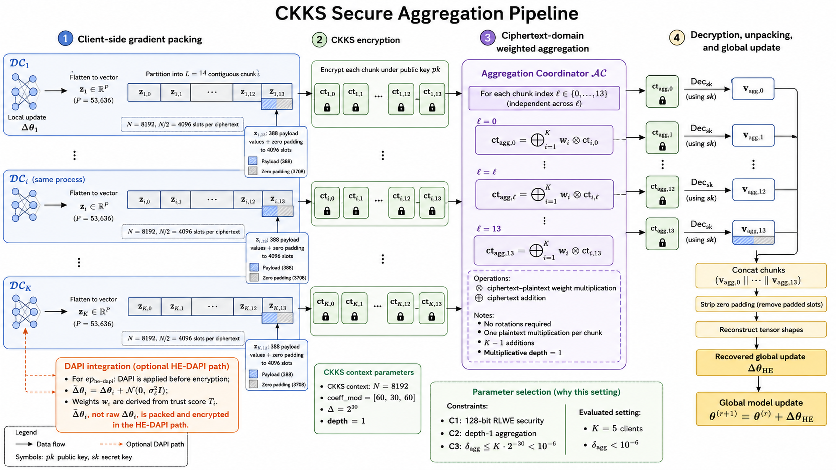
\includegraphics[width=0.50\textwidth,keepaspectratio]{../figures/sec5_sec_agg_ppl.pdf}

  \textbf{Figure~\thefigure.} CKKS aggregation pipeline. Each update is split
  into $L=14$ encrypted chunks and aggregated at $\mathcal{AC}$ with
  plaintext-scalar multiplication and ciphertext addition. $\mathcal{KA}$
  decrypts only the aggregate chunks. Chunks $0$--$12$ contain 4096 payload values;
  chunk~13 contains 388 values and 3708 zeros.
\end{center}

\section{Reproducibility Note}
Source code and scripts are available at:\\
\url{https://github.com/hetiantian10/TWAPPA-FRL} 
and archived on Zenodo at:\\
\url{https://doi.org/10.5281/zenodo.21872240}.

\bibliographystyle{IEEEtran}
\bibliography{../bibliography}

\end{document}
